\documentclass{beamer}
\usepackage[utf8]{inputenc}
\usepackage{graphicx}
\usepackage[T1]{fontenc}

\usetheme{Dresden}
\usecolortheme{dolphin}

\title{Upravljanje sustavom: robotski manipulator \& mobilna baza}
\subtitle{Programiranje mobilnih robota i letjelica (222)}
\author{Filip Bašić \and Joško Jukić \and Ana Šćulac \and \newline Ante Lojić Kapetanović}
\institute[University of Split]{
    Zavod za elektroniku i računarstvo
    @FESB
}
\subject{Mobile robots and drones programming}

\begin{document}

\maketitle

\section{Uvod}

\begin{frame}
    \frametitle{Sadržaj}

    \begin{itemize}
        \item Projektni zadatak\pause
        \item ROS\pause
        \item \emph{Hardware}\pause
        \item Preduvjeti i instalacija\pause
        \item \emph{Software}\pause
        \item Upravljanje\pause
        \item Unaprjeđenja\pause
        \item Literatura
    \end{itemize}
\end{frame}

\begin{frame}
    \frametitle{Projektni zadatak}
    Teleupravljanje mobilnom bazom i robotskim manipulatorom putem web sučelja i \emph{joysticka}:\newline
    \begin{itemize}
        \item Sklopovski povezati paletar s robotskim manipulatorom
        \item Upravljanje obama podsustavima putem bežičnog \emph{joysticka}
        \item Upravljanje obama podsustavima putem web sučelja koje će imati mogućnost video \emph{streama} preko web kamere povezane na robot
        \item Upravljanje ostvariti putem inverznog kinematičkog pristupa
    \end{itemize}
\end{frame}

\section{Osnovne tehnologije i alati}

\begin{frame}
    \frametitle{ROS}
    \begin{columns}
        \column{.6\textwidth}
        Sučelje koje omogućuje upravljanje kompleksnim i heterogenim sklopovljem i aplikacijama, osnovna svojstva:\newline
        \begin{itemize} 
            \item \emph{publisher} - \emph{subscriber} komunikacija preko tema
            \item apstrakcija sklopovlja
            \item instalacija upravljačkih programa
            \item osigurava potrebne bibiloteke
            \item neovisnost o programskom jeziku
        \end{itemize}
        \column{.5\textwidth}
        
\includegraphics{ros.png}
    \end{columns}
\end{frame}

\begin{frame}
    \frametitle{\emph{Hardware} (1)}
    \begin{columns}
        \column{.6\textwidth}
        Robotski manipulator - CPR Mover 4:\newline
        \begin{itemize}
                \item 4 servo zgloba
                \item 550mm dužine uključujući hvataljku (eng. \emph{gripper})
                \item 12V napajanje
                \item ROS manipulacija
        \end{itemize}

        \column{.5\textwidth}
        \begin{figure}[h!]
            \centering
            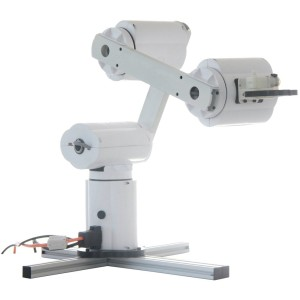
\includegraphics[scale=0.5]{Mover4.jpg}
        \end{figure}
    \end{columns}
\end{frame}

\begin{frame}
    \frametitle{\emph{Hardware} (2)}
    \begin{columns}
        \column{.6\textwidth}
        Robotska mobilna baza - paletar:\newline
        \begin{itemize}
                \item diferencijalni pogon
                \item Linux i ROS instalirani na centralnoj upravljačkoj jedinici
                \item povezan s CPR Mover4 PCAN-USB sučeljem
        \end{itemize}

        \column{.5\textwidth}
        \begin{figure}
            \centering
            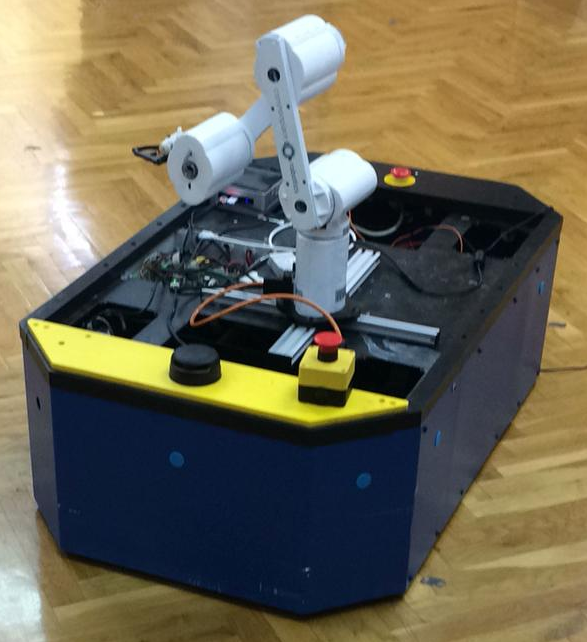
\includegraphics[width=50mm]{paletar.png}
        \end{figure}
    \end{columns}
\end{frame}

\begin{frame}
    \frametitle{Preduvjeti i instalacija}
    Detaljno opisano u dokumentaciji i na antelk/PMRiL @GitHub\newline
    \begin{itemize}
        \item ROS (u našem slučaju Kinematic) instalirati na Linux OS (u našem slučaju Ubuntu 16.04)
        \item PCAN-USB sučelje za komunikaciju Mover4 - paletar
        \item Apache2 server
        \item rosbridge server
        \item roslibjs ROS paket
        \item usb cam ROS paket
        \item joy ROS paket
    \end{itemize}
\end{frame}

\begin{frame}
    \frametitle{\emph{Software}}
    \begin{columns}
        \column{.5\textwidth}
        upravljanje putem \emph{joysticka}
        \begin{itemize}
                \item Python
                \item joy tema registrira pritisak na botun na \emph{joysticku}
                \item joy-concurrent.py očitava koji botun je pritisnut te prema tome manipulira robotom
                \item pomoćne skripte: joy-Mover4.py i joy-paletar.py
        \end{itemize}

        \column{.5\textwidth}
        upraljanje putem web sučelja
        \begin{itemize}
            \item Javascript
            \item ostvaruje komunikaciju između sučelja i sustava preko rosbridge servera
            \item video \emph{stream} ostvaren koristeći usb cam ROS paket
            \item upravljanje je realizirano na način da bilo koja manipulacija kroz sučelje objavljuje formatirane naredbe na odgovarajuće teme
        \end{itemize}

    \end{columns}
\end{frame}

\section{Razvoj}

\begin{frame}
    \frametitle{Upravljanje (1)}
    \begin{columns}
        \column{.5\textwidth}
        Putem \emph{joysticka}:
        \newline onemogućeno istovremeno upravljanje robotskom rukom i paletarom
        \newline\newline Upravljanje s jednog na drugi podsustav se ostvaruje pritiskom na \emph{analog} botun.
        \column{.5\textwidth}
        \begin{figure}[h!]
            \centering
            
\includegraphics[width=50mm]{joy.png}
        \end{figure}
    \end{columns}
\end{frame}

\begin{frame}
    \frametitle{Upravljanje (2)}
    \begin{columns}
        \column{.5\textwidth}
        Putem web sučelja:
        \newline omogućeno istovremeno upravljanje robotskom rukom i paletarom
        \newline\newline Upravljanje robotskom rukom ostvareno kroz sučelje, upravljanje paletarom tipkama w, a, s i d.
        \column{.5\textwidth}
        \begin{figure}[h!]
            \centering
            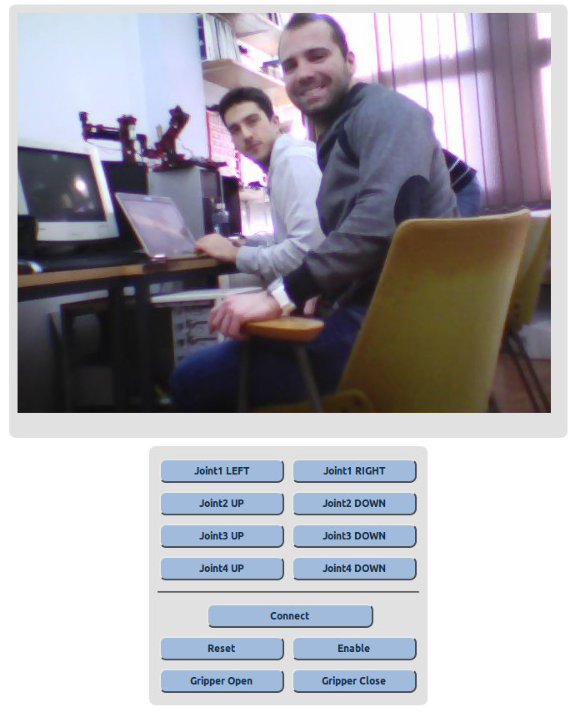
\includegraphics[width=50mm]{web.png}
        \end{figure}
    \end{columns}
\end{frame}

\section{Zaključak}

\begin{frame}
    \frametitle{Unaprjeđenja}
    \begin{itemize}
        \item Implementacija WebRTC za video \emph{stream}
        \item Naprednije upravljanje paletarom
        \item Implementacija tehnike inverzne kinematike za upravljanje robotske ruke
    \end{itemize}
\end{frame}

\begin{frame}
    \frametitle{Literatura}
    
    \begin{thebibliography}{10}
        \beamertemplatearticlebibitems

        \bibitem{wiki}
            Robot OS
            \newblock Wikipedia
        \bibitem{ros}
            Službena ROS dokumentacija
            \newblock wiki.ros.org
        \bibitem{mover}
            Službena Mover4 dokumentacija
            \newblock wiki.cpr-robots.com
    \end{thebibliography}
\end{frame}

\begin{frame}
    Pitanja, pohvale i kritike sada ili na mail (@fesb.hr):\newline
    \begin{itemize}
        \item fbasic00
        \item alojic00
        \item ascula00
        \item jjukic00
    \end{itemize}
    
\end{frame}

\end{document}